\documentclass[11pt]{article}

\usepackage[utf8]{inputenc}
\usepackage[T1]{fontenc}
\usepackage{lmodern}
\usepackage{microtype}
\usepackage{amsmath,amsfonts}
\usepackage{graphicx}
\usepackage{booktabs}
\usepackage{hyperref}
\usepackage{enumitem}
\usepackage{geometry}
\usepackage{parskip}

\geometry{margin=1in}

\title{\textbf{Auditable AI Decision Systems with Bounded Decisions, Explainability, and Confidence Scores}}

\author{
Sankaranarayanan Palamadai Chandrasekaran \\
Simple Machine Mind-sankar@smsquared.ai
}

\date{}

\begin{document}

\maketitle

    \begin{abstract}
    Real-world AI systems must operate under ambiguity and incomplete information. Forcing
    a binary decision when evidence is insufficient produces overconfident and brittle outcomes.
    This work presents an auditable AI decision system with a bounded three-class decision space
    (YES, NO, TBD), structured explainability through auxiliary Human Values (10 labels) and Emotions/Sentiments (28 labels), and per-decision confidence scores. 
    The auxiliary outputs are retained at inference time as control variables for downstream steering, thresholding, and
    reason-code generation. The system is trained on up to 181,000 labeled decision events and
    evaluated on a stratified held-out test split of 22,748 examples (YES: 5,871; NO: 3,159; TBD:
    13,718; majority class TBD at 60.3\%). It achieves Macro F1 = 0.8215 and Accuracy = 0.8485,
    outperforming a majority-action baseline (Macro F1 = 0.2508, Accuracy = 0.6030). Per-class
    F1 scores are 0.8302 (YES), 0.7524 (NO), and 0.8819 (TBD). Inference latency over 200 runs is
    p50 = 200 ms and p95 = 415 ms on an NVIDIA Tesla T4 GPU. These results demonstrate that
    bounded, defer-aware decision control provides a practical and auditable interface for AI systems
    operating under ambiguity and class imbalance. This work argues that bounded, defer-aware
    decision outputs, combined with structured auxiliary signals, form a more reliable and auditable
    interface for AI systems than traditional forced-decision classifiers.
    \end{abstract}

\section{Introduction}

AI systems in production must handle inputs where evidence is incomplete,
contradictory, or insufficient to support confident action. Traditional
classifiers force a hard decision regardless of input quality, producing systems
that are confident by construction but unreliable under ambiguity.
A system that cannot express "not yet determinable" as an explicit output conflates low-confidence
cases with high-confidence ones, degrading reliability and auditability.

Unlike prior approaches that treat abstention as a post-hoc confidence threshold, the TBD class is learned as a first-class outcome, allowing the model to internalize deferral behavior during training rather than relying on external calibration.

A second challenge is that decision outcomes are not determined by input content
alone. The same input may require different handling under different
execution-time conditions—varying risk tolerance, operational constraints, or
deployment context. Systems that do not encode this context cannot adapt without
retraining.

This work addresses both problems through a bounded decision formulation and
structured explainability, and reframes classification as a decision interface
problem rather than a label prediction task. The bounded decision space
$\mathcal{Y}_d = \{\text{YES}, \text{NO}, \text{TBD}\}$ makes deferral an
explicit, auditable output. Unlike prior approaches that treat abstention as a
post-hoc confidence filter on a binary classifier
\cite{elyaniv2010selective, geifman2017selective, franc2023reject}, TBD is
learned as a first-class outcome, enabling the model to internalize when to
defer under uncertainty.

In addition to decision prediction, the system separates decision control by
retaining auxiliary Human Values and Emotions/Sentiments channels at inference
time as structured control variables. These signals encode decision-policy
context and allow downstream systems to apply thresholds, constraints, and
reasoning logic without retraining the model. While multi-task learning
\cite{caruana1997multitask} is typically used for representation sharing, this
work extends it by preserving auxiliary outputs beyond training as an
inference-time explainability and decision-control interface.

\paragraph{Positioning relative to prior work.}
While prior work on selective classification and reject-option models focuses on post-hoc abstention
based on confidence thresholds, these approaches typically treat deferral as an external mechanism
applied after prediction. In contrast, this work incorporates deferral as a learned, first-class
outcome within the model itself, enabling the system to internalize ambiguity during training rather
than relying solely on calibration at inference time.

\noindent\textbf{Contributions:}
\begin{itemize}[leftmargin=1.5em, itemsep=1pt]
  \item A bounded three-class decision formulation (YES/NO/TBD) that treats
        deferral as a first-class trained output, not a confidence-threshold
        artifact.
  \item A multi-task architecture that retains auxiliary explainability outputs
        (Human Values, Emotions/Sentiments) at inference time as structured
        decision-policy control variables.
  \item An empirical evaluation on 22,748 held-out examples with full per-class
        breakdown, confusion matrix, ablation, and latency characterization.
\end{itemize}

\section{System Overview}

The system receives a tokenized decision event, evaluates it through a shared transformer encoder,
and produces three outputs: a bounded decision ($y \in \{\text{YES}, \text{NO}, \text{TBD}\}$), a structured Human
Values vector ($v \in \{0,1\}^{10}$), and a structured Emotions/Sentiments vector ($e \in \{0,1\}^{28}$). All three
outputs are available at inference time. The auxiliary outputs serve as explainability signals and
control variables for downstream reasoning, thresholding, and reason-code generation—they are not
discarded after training.

The model receives a context signal and returns a bounded decision with decision confidence, along with structured reason codes and associated reason-code confidence scores derived from Human Values and Emotions/Sentiments activations.

\begin{figure}[h]
\centering
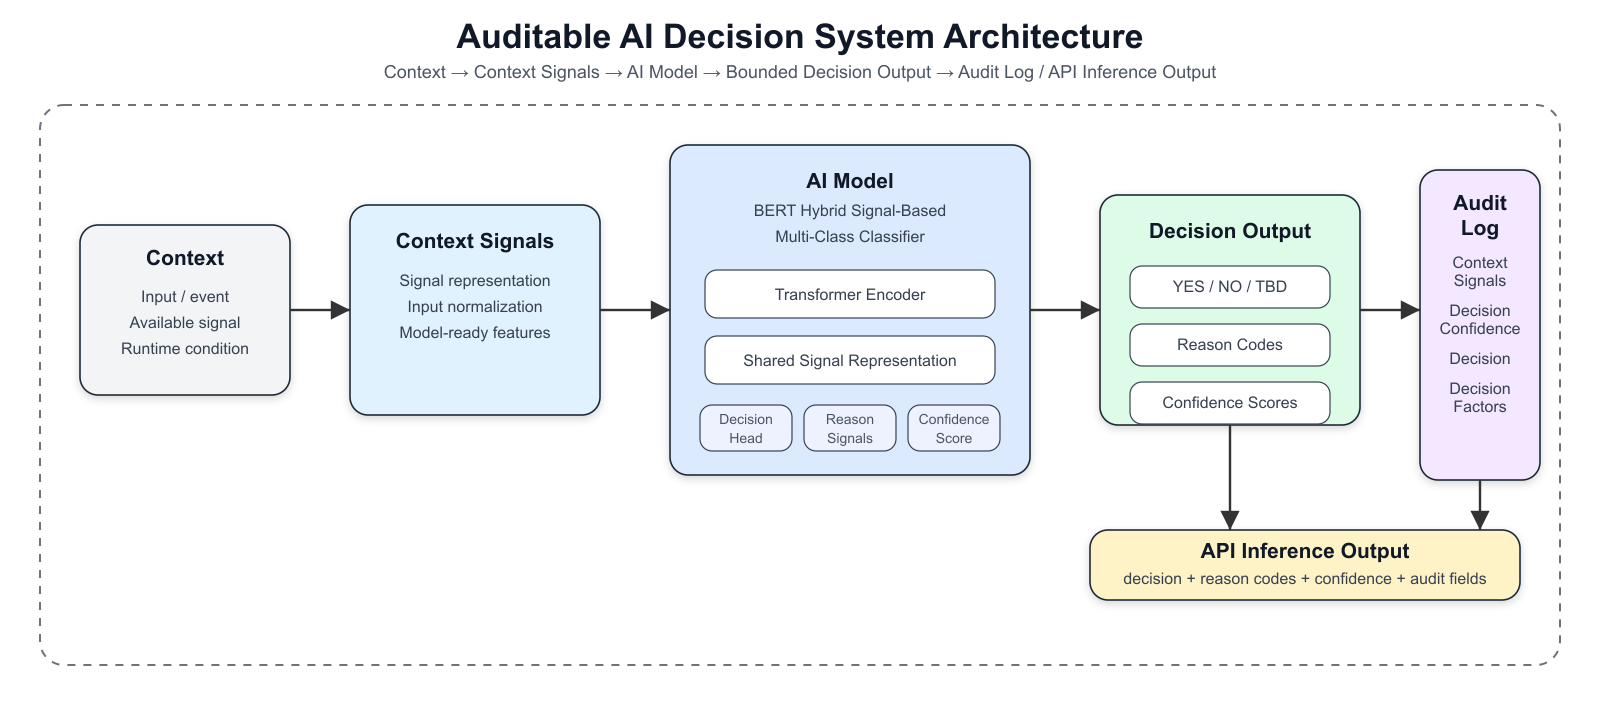
\includegraphics[width=0.9\linewidth]{architecture.png}
\caption{System architecture: tokenized decision event $\to$ shared transformer encoder with auxiliary heads $\to$ bounded decision output with structured explainability outputs (Human Values, Emotions/Sentiments) and confidence score.}
\end{figure}

The full model jointly predicts $f(x) = (f_d(x), f_v(x), f_e(x))$, where $f_d$ is the bounded decision
function and $f_v$, $f_e$ are the auxiliary context functions retained for inference-time control.

\section{Methodology}

\subsection{Architecture}

The model uses a transformer-based multi-task architecture initialized from bert-base-uncased
\cite{devlin2019bert}. A shared encoder processes tokenized inputs (maximum 128 tokens) and produces a contextual
representation consumed by three task-specific output heads:

\begin{itemize}
\item Decision head: three-class classifier producing $y \in \{\text{YES}, \text{NO}, \text{TBD}\}$.
\item Value head: 10-label multi-label predictor for Human Values.
\item Emotion head: 28-label multi-label predictor for Emotions/Sentiments.
\end{itemize}

Confidence scores are derived from the primary decision head softmax and exposed at inference
alongside the auxiliary outputs. Calibration of neural classifier confidence is a known challenge
\cite{guo2017calibration}; the TBD class provides a native low-confidence route independent of softmax calibration.

\subsection{Training}

The model is trained jointly on the primary bounded decision task and the two auxiliary multi-label
tasks under the following configuration:

\begin{itemize}
\item Backbone: bert-base-uncased; maximum sequence length: 128 tokens
\item Batch size: 32
\item Learning rate: layer-wise differential rates across encoder layers and task-specific heads; cosine decay with warmup ratio 0.1
\item Random seed: 42
\item Class imbalance handling: per-class decision weights applied to the primary head loss
\end{itemize}

This joint formulation ensures that decision outputs, auxiliary signals, and confidence scores are
learned from a shared representation, enabling consistent behavior across prediction, explanation,
and downstream control.

\section{Results and Analysis}

\subsection{Dataset and Evaluation Setup}

The corpus contains up to 181,000 labeled decision events. Each example carries a primary bounded
decision label (YES/NO/TBD) and multi-label annotations for Human Values (10 labels) and
Emotions/Sentiments (28 labels). Results are reported on a stratified held-out test split of 22,748
examples:

\paragraph{Dataset provenance and construction.}
The corpus was constructed by combining multiple public NLP datasets into a unified decision-event
format and applying data-quality filtering to produce a curated set of up to 181,000 labeled
examples. All listed source datasets were used in corpus construction. The sources include
SemEval-2017 \cite{rosenthal2017semeval}, Financial PhraseBank \cite{malo2014good},
TweetEval and TweetEval Health \cite{barbieri2020tweeteval}, GoEmotions
\cite{demszky2020goemotions}, NormBank \cite{ziems2023normbank},
Moral Foundations-style value data \cite{hoover2020mftc}, MELD \cite{poria2019meld},
Empathetic Dialogues \cite{rashkin2019empathetic}, Social Bias Frames
\cite{sap2020socialbias}, ETHICS and virtue-oriented ethics data
\cite{hendrycks2021ethics}, Sentiment140 \cite{go2009twitter}, IMDb
\cite{maas2011learning}, and MultiNLI \cite{williams2018broad}.

The source datasets cover complementary signal types: sentiment and stance-like classification,
emotion recognition, dialogue context, social and normative reasoning, natural language inference,
ethical judgment, and human-value framing. These heterogeneous sources were normalized into a
common representation in which each example is treated as a decision event with a primary bounded
decision label (YES, NO, or TBD), a 28-label Emotions/Sentiments vector, and a 10-label Human
Values vector.

The resulting dataset should be interpreted as a curated research corpus for evaluating bounded
decision behavior rather than as a single naturally occurring production dataset. The construction
process is intended to expose the model to clear positive, clear negative, and ambiguity-heavy
contexts so that the model can learn the boundary between action, rejection, and deferral.

\begin{center}
\begin{tabular}{lrr}
\toprule
Class & Count & Share \\
\midrule
YES & 5,871 & 25.8\% \\
NO & 3,159 & 13.9\% \\
TBD & 13,718 & 60.3\% \\
Total & 22,748 & 100.0\% \\
\bottomrule
\end{tabular}
\end{center}

TBD is the majority class (60.3\%), so Macro F1 is the primary evaluation metric.

\subsection{Auxiliary Label Spaces}

\paragraph{Human Values label space.}
The Human Values auxiliary head follows the classic 10-value taxonomy from Schwartz's Theory of
Basic Human Values \cite{schwartz2012overview}: Self-Direction, Stimulation, Hedonism,
Achievement, Power, Security, Conformity, Tradition, Benevolence, and Universalism. These values
represent broad motivational goals that can shape how a decision context is interpreted.

In this system, Human Values labels are used as multi-label context descriptors rather than as
standalone moral judgments. A decision event may activate multiple value dimensions simultaneously.
For example, a case involving potential harm and institutional rules may activate Security,
Conformity, or Benevolence-related signals, while a case involving independent choice may activate
Self-Direction. These signals are retained at inference time to support auditability, policy
thresholds, and reason-code generation.

\paragraph{Emotions/Sentiments label space.}
The Emotions/Sentiments auxiliary head follows the 28-label GoEmotions taxonomy. The labels are:
admiration, amusement, anger, annoyance, approval, caring, confusion, curiosity, desire,
disappointment, disapproval, disgust, embarrassment, excitement, fear, gratitude, grief, joy, love,
nervousness, optimism, pride, realization, relief, remorse, sadness, surprise, and neutral.

These labels capture affective and sentiment-bearing context that may influence the interpretation
of a decision event. They are not treated as causal explanations of the bounded decision output.
Instead, they provide structured context that downstream systems can inspect when applying
thresholds, routing decisions, or generating reason codes.

\subsection{Performance Comparison}

\begin{center}
\begin{tabular}{lcccc}
\toprule
Method & Accuracy & Macro F1 & Micro F1 & Weighted F1 \\
\midrule
Majority-action baseline (always TBD) & 0.6030 & 0.2508 & 0.6030 & 0.4537 \\
Bounded-decision ablation & -- & 0.8211 & -- & -- \\
Proposed system & 0.8485 & 0.8215 & 0.8485 & 0.8506 \\
\bottomrule
\end{tabular}
\end{center}

\subsection{Per-Class Performance}

\begin{center}
\begin{tabular}{lrrrr}
\toprule
Class & Precision & Recall & F1 & Support \\
\midrule
YES & 0.7683 & 0.9029 & 0.8302 & 5,871 \\
NO & 0.7164 & 0.7923 & 0.7524 & 3,159 \\
TBD & 0.9306 & 0.8381 & 0.8819 & 13,718 \\
\bottomrule
\end{tabular}
\end{center}

\subsection{Confusion Matrix}

\begin{center}
\begin{tabular}{lccc}
\toprule
 & Pred YES & Pred NO & Pred TBD \\
\midrule
True YES & 5,301 & 141 & 429 \\
True NO & 228 & 2,503 & 428 \\
True TBD & 1,371 & 850 & 11,497 \\
\bottomrule
\end{tabular}
\end{center}

\subsection{Inference Latency}

Measured over 200 inference runs on NVIDIA Tesla T4 (16 GB): p50 = 200 ms, p95 = 415 ms.

\subsection{Qualitative Example}

To illustrate the behavior of the bounded decision system, we provide a representative example of a
decision event and its associated outputs.

\noindent\textbf{Input:}
\begin{quote}
The user expresses uncertainty about proceeding with a financial investment given conflicting advice
and potential risk.
\end{quote}

\noindent\textbf{Model Output:}
\begin{itemize}[leftmargin=1.5em, itemsep=1pt]
  \item Decision: TBD
  \item Confidence: 0.62
  \item Human Values (top activations): Security, Conformity
  \item Emotions/Sentiments (top activations): confusion, nervousness
\end{itemize}

In this case, the model assigns a TBD outcome, reflecting insufficient confidence to recommend a
definitive action. The auxiliary signals indicate a context involving risk sensitivity (Security),
adherence to norms (Conformity), and emotional uncertainty (confusion, nervousness).

Rather than forcing a YES or NO decision, the system explicitly represents ambiguity and exposes
structured signals that downstream systems can use for escalation, additional data collection, or
policy-based routing.

\section{Discussion}

The 0.5707 Macro F1 improvement over the majority-action baseline confirms that
the model learns genuine three-way discrimination rather than exploiting class
imbalance. The TBD class constitutes 60.3\% of the test split; a system
predicting TBD exclusively achieves 60.3\% accuracy. The proposed system
reaches 84.9\% accuracy with strong coverage across all three decision states.

The ablation result (0.0019 Macro F1 gap) shows that the auxiliary channels are
not the primary source of classification performance. Their operational value is
at inference time: the Human Values and Emotions/Sentiments outputs allow
downstream systems to inspect decision-policy context, apply deployment-specific
thresholds, and generate structured reason codes without modifying the core
model.

The dominant error mode—true TBD predicted as YES—highlights the boundary between
action and deferral. This boundary can be tuned at deployment time using
confidence scores and auxiliary signals, providing a practical mechanism for
risk-sensitive decision control.

More broadly, this formulation reframes classification from a forced labeling
problem into a decision interface problem, where abstention, explanation, and
confidence are co-equal outputs. This shift is particularly relevant for systems
deployed under uncertainty, where the cost of incorrect action exceeds the cost
of deferral.

\section{Limitations}

Results are specific to the dataset, label spaces, and evaluation environment used in this study.
While the decision formulation and signal-based representation are designed to be domain-agnostic,
empirical validation across additional decision domains remains an area for future work.
Class imbalance in the NO class (13.9\% of the test split) likely constrains NO performance 
and may require additional data or targeted loss shaping. Reported latency figures are hardware-dependent.
Fuller isolation of individual auxiliary channel contributions to bounded decision behavior is
deferred to future work.

\paragraph{Scope of claims.}
The results suggest that bounded decision outputs can provide a practical approach to representing
uncertainty in AI decision systems. They demonstrate potential for defer-aware decision control in a
curated decision-event corpus constructed from heterogeneous public NLP datasets. The results should
not be interpreted as proving universal generalization across all domains or deployment settings.

The auxiliary Human Values and Emotions/Sentiments heads provide structured context signals rather
than complete explanations of model behavior. They support auditability and downstream control, but
deployment in a new domain should include separate validation of label behavior, calibration, class
balance, and operational thresholds.

\paragraph{Reproducibility and implementation details.}
The implementation described in this work is based on standard transformer architectures and
publicly available datasets. Additional implementation details, including data preprocessing steps,
training configuration, and evaluation scripts, can be made available upon request to support
reproducibility and further research.

\paragraph{Artifact availability.}
Project artifacts, documentation, model-card materials, and publication support files are maintained
in the public repository at \url{https://github.com/pcsankar73/EvaluatorDPT-Publish}. The associated
model card is available at \url{https://huggingface.co/pcsankar73s/EvaluatorModel}.

\section{Conclusion}

This paper presented an auditable AI decision system with bounded decisions
(YES/NO/TBD), structured explainability through auxiliary Human Values and
Emotions/Sentiments outputs, and per-decision confidence scores. On a stratified
held-out test split of 22,748 examples from a corpus of up to 181,000 labeled
decision events, the system achieves Macro F1 = 0.8215 and Accuracy = 0.8485,
outperforming a majority-action baseline by 0.5707 Macro F1 points. Per-class
F1 scores are 0.8302 (YES), 0.7524 (NO), and 0.8819 (TBD). An ablation
confirms that auxiliary channels contribute inference-time control variables
rather than classification gain. Inference latency is p50 = 200 ms and
p95 = 415 ms on an NVIDIA Tesla T4 GPU.

Beyond performance improvements, this work introduces a shift from forced classification 
toward decision interfaces that explicitly incorporate deferral, explainability, 
and confidence as first-class outputs. By separating decision prediction from decision 
control, the system enables execution-time adaptation without retraining, allowing 
downstream systems to apply thresholds, policies, and constraints dynamically. 
The bounded decision formulation ensures that uncertainty is represented explicitly 
rather than suppressed, while auxiliary signals provide a structured and auditable basis 
for interpreting and steering decisions. This combination positions the system not merely 
as a classifier, but as a practical decision control layer for real-world AI deployments 
operating under uncertainty.

\bibliographystyle{plain}
\bibliography{references}

\end{document}
